%!TEX TS-program = xelatex
%\documentclass[newPxFont]{beamer}
%\documentclass[newPxFont,handout]{beamer} % Раздаточный материал (на слайдах всё сразу)
\documentclass[aspectratio=169]{beamer} % Соотношение сторон


\usetheme{LTX}

%-=-=-=-=-=-=-=-=-=-=-=-=-=-=-=-=-=-=-=-=-=-=-=-=
%        LOADING PACKAGES
%-=-=-=-=-=-=-=-=-=-=-=-=-=-=-=-=-=-=-=-=-=-=-=-=
\usepackage{amsmath,amsfonts,amssymb,amsthm,mathtools}  % Тут мы подключаем пакеты для математики!
\usepackage{wasysym}
%%%%%%%%%%%%%%%%%%%%%%%% Шрифты %%%%%%%%%%%%%%%%%%%%%%%%%%%%%%%%%

\usepackage{fontspec}         % пакет для подгрузки шрифтов
\setmainfont{Helvetica}  % задаёт основной шрифт документа

% why do we need \newfontfamily:
% http://tex.stackexchange.com/questions/91507/
\newfontfamily{\cyrillicfonttt}{Helvetica}
\newfontfamily{\cyrillicfont}{Helvetica}
\newfontfamily{\cyrillicfontsf}{Helvetica}
% Иногда тех не видит структуры шрифтов. Эти трое бравых парней спасают ситуацию и доопределяют те куски, которые Тех не увидел.

% \usepackage{unicode-math}     % пакет для установки математического шрифта
% \setmathfont{Asana Math}      % шрифт для математики

\usepackage{polyglossia}      % Пакет, который позволяет подгружать русские буквы
\setdefaultlanguage{russian}  % Основной язык документа
\setotherlanguage{english}    % Второстепенный язык документа

%%% Работа с картинками
\usepackage{graphicx}  % Для вставки рисунков
\graphicspath{{images/}{images2/}}  % папки с картинками
\setlength\fboxsep{3pt} % Отступ рамки \fbox{} от рисунка
\setlength\fboxrule{1pt} % Толщина линий рамки \fbox{}
\usepackage{wrapfig} % Обтекание рисунков текстом

%%% Работа с таблицами
\usepackage{array,tabularx,tabulary,booktabs} % Дополнительная работа с таблицами
\usepackage{longtable}  % Длинные таблицы
\usepackage{multirow} % Слияние строк в таблице

%%% Программирование
\usepackage{etoolbox} % логические операторы

%%% Другие пакеты
\usepackage{multicol} % Несколько колонок

%%% Картинки
\usepackage{tikz} % Работа с графикой
\usepackage{pgfplots}
\usepackage{pgfplotstable}


\usepackage{xcolor}
\usepackage{hyperref}
\hypersetup{				
    unicode=true,           % позволяет использовать юникодные символы
    colorlinks=true,       	% true - цветные ссылки, false - ссылки в рамках
    urlcolor=blue,          % цвет ссылки на url
    linkcolor=red,          % внутренние ссылки
	hyperindex=true,        % сделать ли ссылку кликабельной?
	breaklinks=true         % если ссылка не умещается в одну строку, разбивать    
	                        % ли ее на две части?
}
\usepackage{verbatim}
\usepackage{fancyvrb}
\usepackage{mdframed}

 
\usepackage{chronology}

\renewcommand{\event}[3][e]{%
  \pgfmathsetlength\xstop{(#2-\theyearstart)*\unit}%
  \ifx #1e%
    \draw[fill=black,draw=none,opacity=0.5]%
      (\xstop, 0) circle (.2\unit)%
      node[opacity=1,rotate=45,right=.2\unit] {#3};%
  \else%
    \pgfmathsetlength\xstart{(#1-\theyearstart)*\unit}%
    \draw[fill=black,draw=none,opacity=0.5,rounded corners=.1\unit]%
      (\xstart,-.1\unit) rectangle%
      node[opacity=1,rotate=45,right=.2\unit] {#3} (\xstop,.1\unit);%
  \fi}%


\title{Уютный факультатив по \LaTeX}
\subtitle{Шрифты, документ в целом, преамбула для души}
\date{\today}

\begin{document}

\begingroup
\setbeamercolor{background canvas}{bg = LTXDarkGrey}
\begin{frame}[plain]
\centering  
\includegraphics[width=0.63\linewidth]{font.jpg}	
\end{frame}
\endgroup 

\maketitle


\begin{frame}{Agenda} 
\begin{itemize}
	\item Как латех прокрался в ворд
	\item Для извращенцев: из Wolfram в \LaTeX{ }
	\item Про шрифты, юникод, рыцарей и о тех, кто попадает в ад
	\item Графика в техе, контракт по продаже души
	\item Снова про картинки, опять про таблицы
\end{itemize}
\end{frame}


\section{Шрифты}  



\begin{frame}{Кодировка} 
Кодировка - способ представления в памяти компьютера цифр, букв и всех остальных знаков. 

\centering 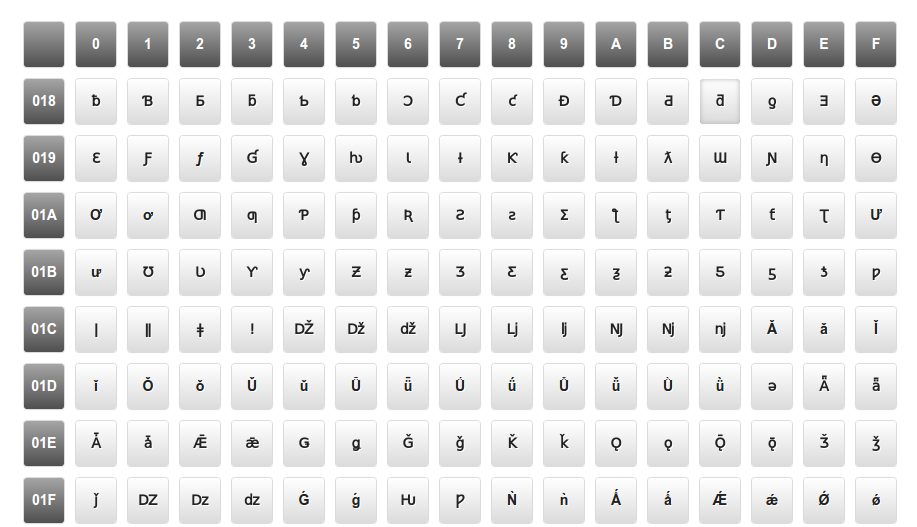
\includegraphics[width=0.68\linewidth]{codirovka.png}	
\end{frame}

\begin{frame}{Откуда берутся кракозябры} 
\centering 
\includegraphics[width=0.7\linewidth]{krakozabr.jpg}	
\vspace{0.3cm}

\begin{itemize}
\item Мало памяти, 7 бит достаточно для всего (256 ячеек)
\item 127 ячеек - основа: символы, цифры, латиница
\item 128 ячеек - другое: кириллица, немецкий и т.п.
\item Каждое новое заполнение 128 символов $\Rightarrow$ новая кодировка
\end{itemize}
\end{frame}


\begin{frame}{Юникод} 
\begin{itemize}
\item Собрались великие умы в 1991 году и юникод придумали!
\end{itemize}

\centering  
\includegraphics[width=0.7\linewidth]{stdcom.jpg}	
\end{frame}


\begin{frame}{Мольба к аудитории}
\begin{columns}
\begin{column}{.66\linewidth}
\Large Весь мир уже давно перешёл на utf-8! Будьте прогрессивными! Плиз... 
\end{column}
\begin{column}{.33\linewidth}
\hfill 
\includegraphics[width=\linewidth]{cuputf8.jpg}	
\end{column}
\end{columns}
\end{frame}


{
\usebackgroundtemplate{%
\tikz\node[opacity=0.15] {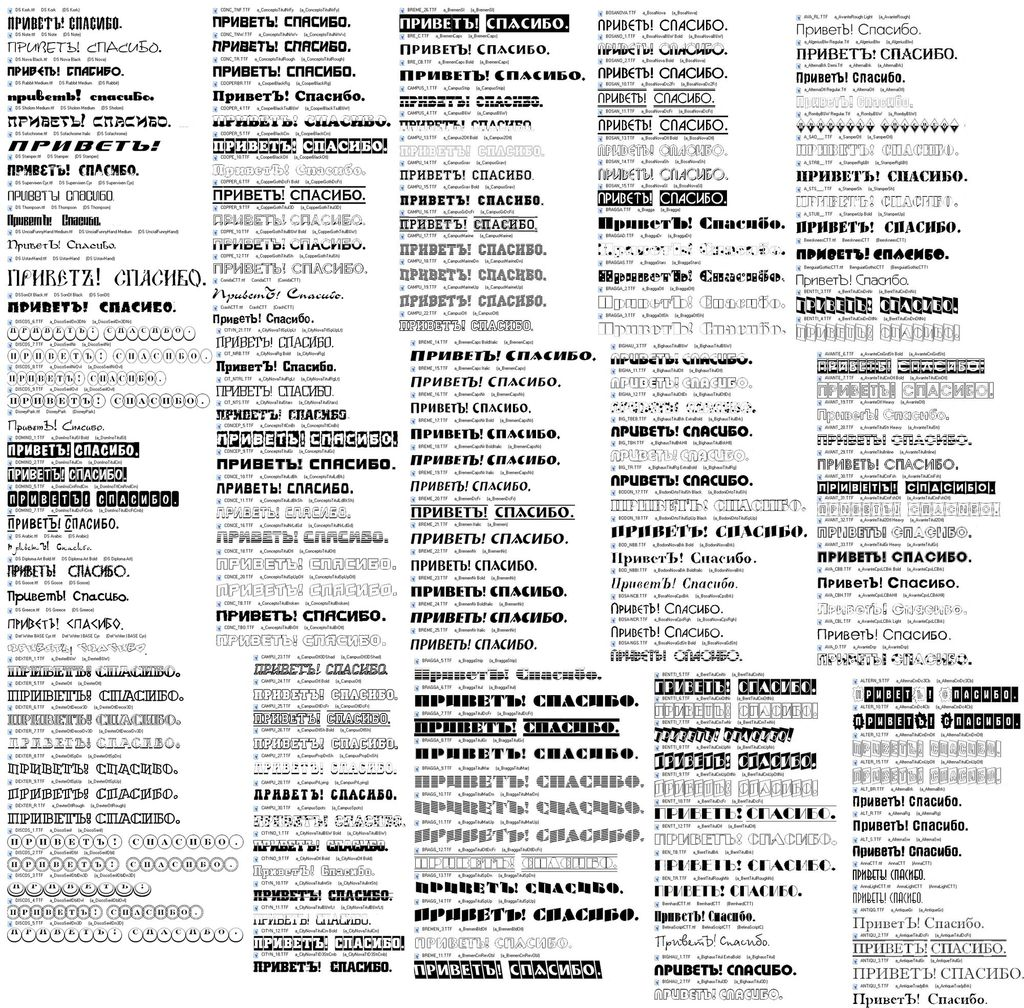
\includegraphics[width=\paperwidth]{bakcfont.jpg}};}
\begin{frame}{Откуда берутся шрифты}
\Large
\begin{itemize}
\item Шрифты скачиваются из интернета \ldots
\item Хорошая идея - установить на комп шрифтовый менеджер для безболезненного просмотра шрифтов
%\item Хороший \href{https://apps.ubuntu.com/cat/applications/precise/font-manager/}{ шрифтовый менеджер} для Linux 
\item Наверное, неплохой \href{http://fontba.se/}{ шрифтовый менеджер}
\end{itemize}
\end{frame}
}

% Показываю файл со шрифтами и их подключением, виньетки для fontspect и для math-unicode
% Показать ссылки на документацию пакетов
% https://www.ctan.org/pkg/fontspec
% https://www.ctan.org/pkg/unicode-math

\begin{frame}[fragile]{Первые строки преамбулы}
\begin{block}{  }
\verb|   \usepackage[british,russian]{babel}   % выбор языка| \newline
\verb|   \usepackage[utf8]{inputenc}               % utf8 кодировка| \newline
\verb|   \usepackage[X2,T2A]{fontenc}           % ещё кодировка|
\end{block}

\begin{itemize}
\item Если вы где-то увидели \verb|\usepackage[cp1251]{inputenc}|,  замените  на  \verb|\usepackage[utf8]{inputenc}|
\end{itemize}
\end{frame}

\begin{frame}{Задание 1} 
\begin{enumerate}
	\item  Открыть файлик  \texttt{xetex fonts.tex}
	\item  Скачать и установить все требуемые шрифты
	\item  Убедиться, что документ создаётся
	\item  Попробовать поставить шрифт бандитов как математический, посмотреть что будет и попробовать это объяснить
\end{enumerate}
\end{frame}


\begin{frame}[fragile]{Матшрифты}

\begin{itemize}
\item \href{http://ftp.math.purdue.edu/mirrors/ctan.org/macros/latex/contrib/unicode-math/unimath-symbols.pdf}{Разные матшрифты}
\end{itemize}

\begin{center}
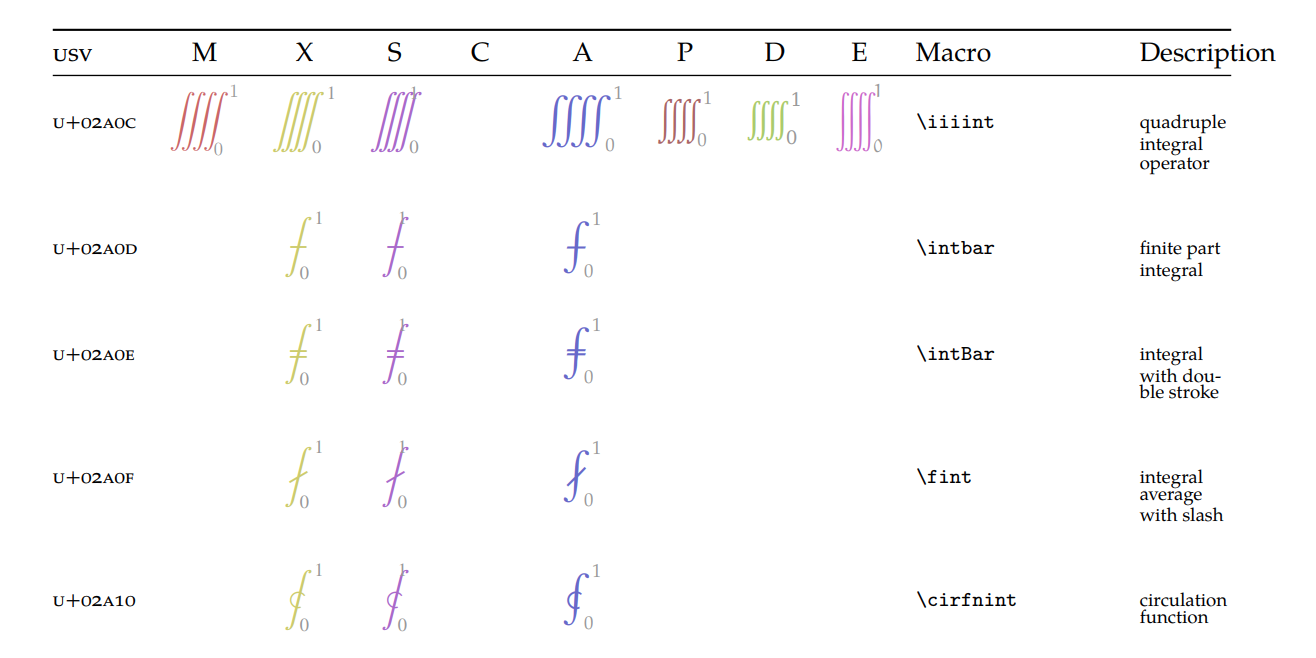
\includegraphics[width=0.8\linewidth]{math_fonts.png}
\end{center}	
\end{frame}

{
	\usebackgroundtemplate{%
		\tikz\node[opacity=1] {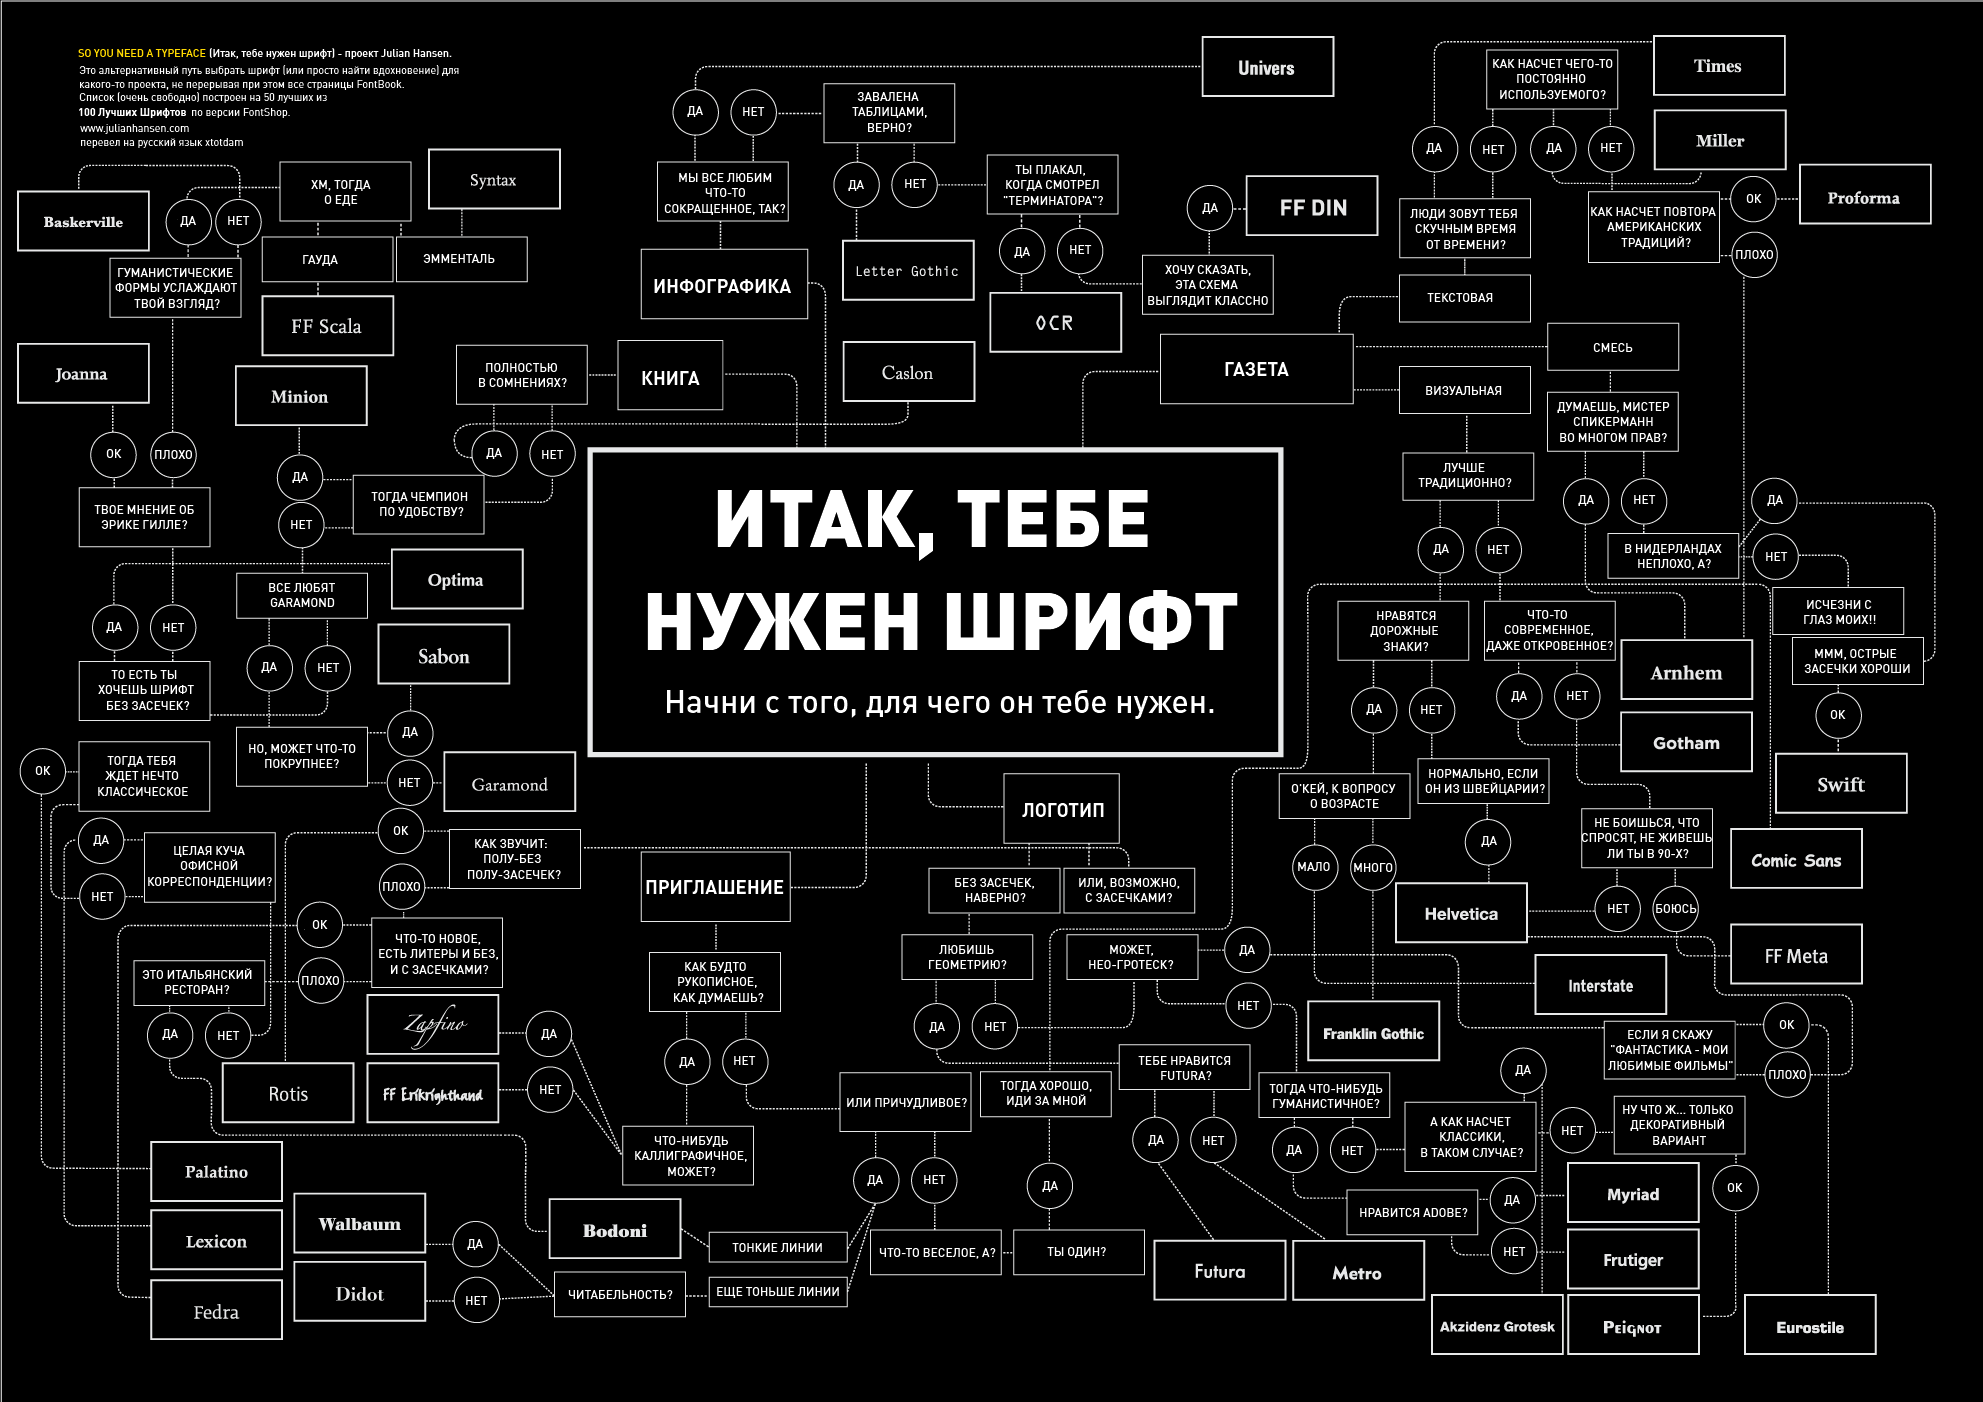
\includegraphics[width=\paperwidth]{fonts.png}};}
\begin{frame}
\end{frame}
}



\section{Таблицы (опять) и картинки (снова)} 

% показать как в texmaker вставлять шаблон с таблицей! Quick Tabular

\begin{frame}
\begin{block}{Типы колонок в таблицах}
\centering 
	\begin{tabulary}{\textwidth}{JL}
		\toprule
			c & колонка выровнена по центру \\
			l & колонка выровнена по левому краю\\
			r & колонка выровнена по правому краю\\
	   p\{ \} & колонка создаётся как абзац, в скобках ширина колонки \\
		   X  & подбирает столбцы равной ширины (tabularx) \\
		   C  & одинаково строк во всех столбцах, выравнивание по центру  \\	  
		   J  & одинаково строк во всех столбцах, выравнивание по ширине \\
		   R  & одинаково строк во всех столбцах, выравнивание по правому краю \\
		   L  & одинаково строк во всех столбцах, выравнивание по левому краю  \\
		\bottomrule
	\end{tabulary}
\end{block}
\vspace{0.1cm} \centering
\large Последние четыре команды лежат в пакете tabulary

\alert{Не забывайте о существовании Quick Tabular \ldots}

\end{frame}

\begin{frame}{Читаемые и нечитаемые таблицы} 
\begin{columns}
\begin{column}{.49\linewidth}
\tiny
\begin{tabular}{|r|r|r|r|r|}
\hline
& Estimate & Std. Error & t value & $Pr( > | t |)$ \\
\hline
Intercept & -1.6598 & 0.0239 & -69.51 & 0.0000 \\ \hline
cut & -0.0206 & 0.0014 & -14.53 & 0.0000 \\ \hline
color & 0.1085 & 0.0011 & 97.30 & 0.0000 \\ \hline
clarity & -0.1784 & 0.0021 & -86.67 & 0.0000 \\ \hline
depth & 0.0121 & 0.0003 & 43.28 & 0.0000 \\ \hline
table & 0.0022 & 0.0002 & 12.07 & 0.0000 \\ \hline
price & 0.0000 & 0.0000 & 231.49 & 0.0000 \\ \hline
x & 0.2425 & 0.0018 & 134.73 & 0.0000 \\ \hline
y & 0.0060 & 0.0012 & 4.92 & 0.0000 \\ \hline
z & 0.0046 & 0.0021 & 2.18 & 0.0290 \\ 
\hline
\end{tabular}
\end{column}
\begin{column}{.49\linewidth}
\tiny
\begin{tabular}{rrrrr}
\toprule
& Estimate & Std. Error & t value & $Pr( > | t |)$ \\
\midrule
Intercept & -1.6598 & 0.0239 & -69.51 & 0.0000 \\ 
cut & -0.0206 & 0.0014 & -14.53 & 0.0000 \\ 
color & 0.1085 & 0.0011 & 97.30 & 0.0000 \\ 
clarity & -0.1784 & 0.0021 & -86.67 & 0.0000 \\ 
depth & 0.0121 & 0.0003 & 43.28 & 0.0000 \\ 
table & 0.0022 & 0.0002 & 12.07 & 0.0000 \\ 
price & 0.0000 & 0.0000 & 231.49 & 0.0000 \\ 
x & 0.2425 & 0.0018 & 134.73 & 0.0000 \\
y & 0.0060 & 0.0012 & 4.92 & 0.0000 \\
z & 0.0046 & 0.0021 & 2.18 & 0.0290 \\ 
\bottomrule
\end{tabular}
\end{column}
\end{columns}

\vspace{1cm}
\centering
\Large
\alert{Какая из таблиц лучше? Выбор очевиден?} 
\end{frame}


\begin{frame}{Ещё пример} 
\centering
\tiny
\begin{tabular}{|c|c|c|c|c|c|c|c|} 
\hline
$m$ & $\Re\{\underline{\mathfrak{X}}(m)\}$ &$-\Im\{\underline{\mathfrak{X}}(m)\}$ & $\mathfrak{X}(m)$ & $\frac{\mathfrak{X}(m)}{23}$ & $A_m$ & $\varphi(m)\ /\ ^{\circ}$ & $\varphi_m\ /\ ^{\circ}$ \\ \hline
1  & 16.128 & +8.872 & 16.128 & 1.402 & 1.373 & -146.6 & -137.6 \\  \hline
2  & 3.442  & -2.509 & 3.442  & 0.299 & 0.343 & 133.2  & 152.4  \\  \hline
3  & 1.826  & -0.363 & 1.826  & 0.159 & 0.119 & 168.5  & -161.1 \\  \hline
4  & 0.993  & -0.429 & 0.993  & 0.086 & 0.08  & 25.6   & 90     \\  \hline
5  & 1.29   & +0.099 & 1.29   & 0.112 & 0.097 & -175.6 & -114.7 \\  \hline
6  & 0.483  & -0.183 & 0.483  & 0.042 & 0.063 & 22.3   & 122.5  \\  \hline
7  & 0.766  & -0.475 & 0.766  & 0.067 & 0.039 & 141.6  & -122   \\  \hline
\end{tabular}

\Large{\alert{И выбор снова очевиден!}}

\tiny
\begin{tabular}{cccccccc} \toprule
    {$m$} & {$\Re\{\underline{\mathfrak{X}}(m)\}$} & {$-\Im\{\underline{\mathfrak{X}}(m)\}$} & {$\mathfrak{X}(m)$} & {$\frac{\mathfrak{X}(m)}{23}$} & {$A_m$} & {$\varphi(m)\ /\ ^{\circ}$} & {$\varphi_m\ /\ ^{\circ}$} \\ \midrule
1  & 16.128 & +8.872 & 16.128 & 1.402 & 1.373 & -146.6 & -137.6 \\
 2  & 3.442  & -2.509 & 3.442  & 0.299 & 0.343 & 133.2  & 152.4  \\
 3  & 1.826  & -0.363 & 1.826  & 0.159 & 0.119 & 168.5  & -161.1 \\
4  & 0.993  & -0.429 & 0.993  & 0.086 & 0.08  & 25.6   & 90     \\
5  & 1.29   & +0.099 & 1.29   & 0.112 & 0.097 & -175.6 & -114.7 \\
6  & 0.483  & -0.183 & 0.483  & 0.042 & 0.063 & 22.3   & 122.5  \\
7  & 0.766  & -0.475 & 0.766  & 0.067 & 0.039 & 141.6  & -122   \\ \bottomrule
\end{tabular}
\end{frame}


\begin{frame}{Правила этикета для истиных Леди и Джентельменов} 
\begin{block}{Заповеди из документации к booktabs}
\begin{enumerate}
\item Будьте проще! Глазам должно быть комфортно.
\item Не используйте вертикальные линни.
\item Не используйте двойные линии. Как правило достаточно трёх горизонтальных линий.
\item Оставляйте место между строками
\item Единицы измерения - в шапку таблицы
\item Повторяющееся значение повторяйте, а не говорите "то же"
\item Если сомневаетесь, выравнивайте по левому краю!
\end{enumerate}
\end{block}
\end{frame}


\begin{frame}[plain]{Задание 2} 
%\begin{center} 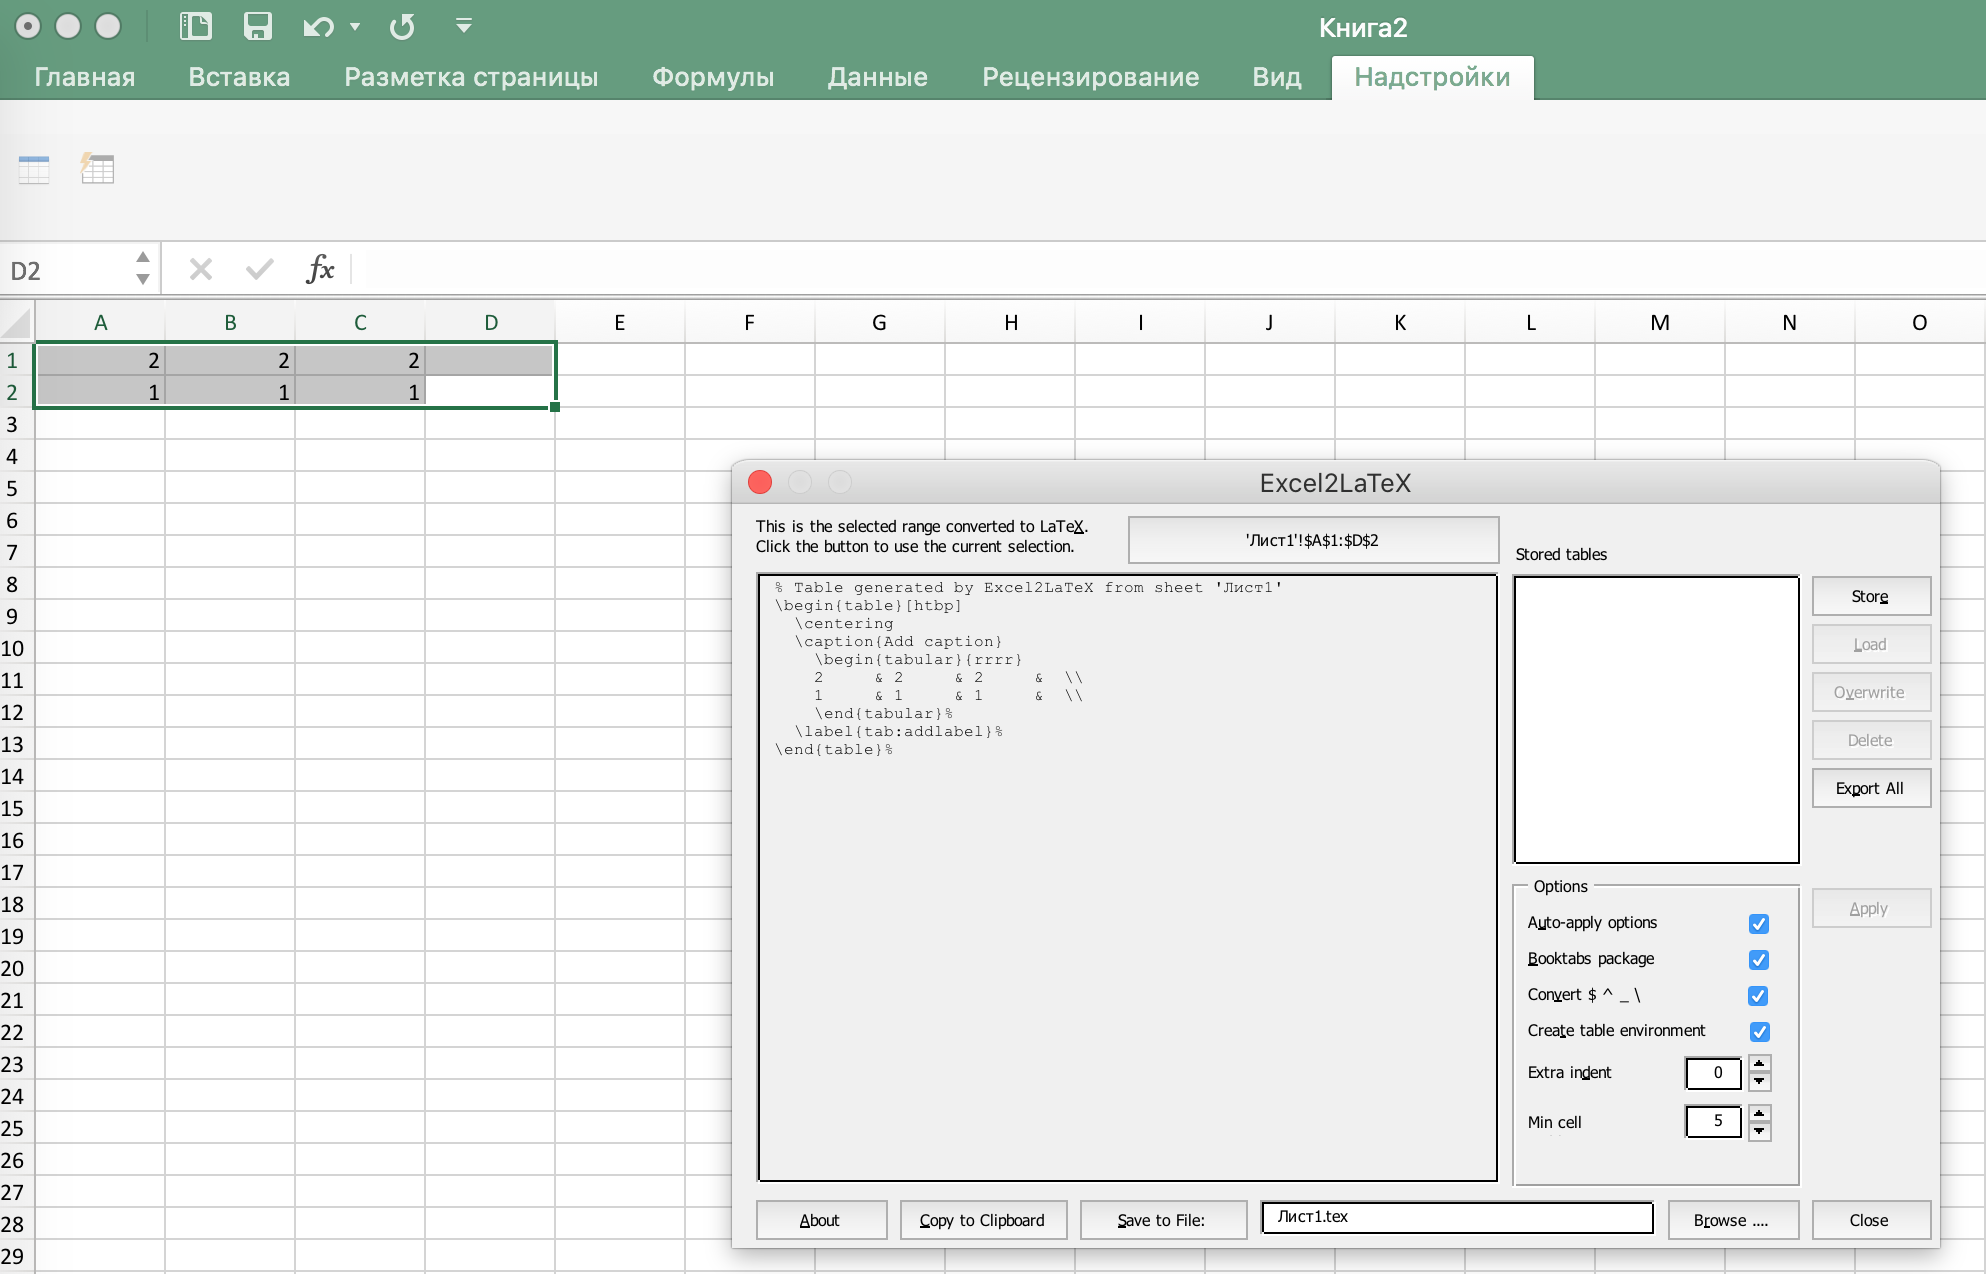
\includegraphics[width=0.45\linewidth]{excel2latex.png}	
%\end{center}

\begin{enumerate}
	\item  Создать свежий файл и скопировать преамбулу для таблиц/рисунков
	\item  Установить надстройку
	\item  Создать любую таблицу и перенести её в \LaTeX
	\item  Сделать таблицу нумеруемой, подписать
	\item  Попробовать объединить какие-нибудь две ячейки в одну
	\item  Если вы самый умный то попробуйте перетащить таблицу из R 
\end{enumerate}

\begin{block}{Ссылка на макрос Excel2LaTeX:}
	\vspace{3mm}
	\centerline {\url{https://ctan.org/tex-archive/support/excel2latex}}
	\vspace{3mm}
\end{block}
\end{frame}

\section{Документ в целом} 

\section{Словари} 

 \begin{frame}[plain]{Установка словарей (орфография)}
 
 \begin{block}{Пошаговая инструкция:}
 	\vspace{3mm}
 	\centerline {\url{ http://blog.harrix.org/article/656}}
 	\vspace{3mm}
 \end{block}
\end{frame}

\begingroup
\setbeamercolor{background canvas}{bg = LTXDarkGrey}
\begin{frame}[plain]
\centering 
\includegraphics[width=0.55\linewidth]{wearlatex.png}
\end{frame}
\endgroup 
\end{document}
